\section{Chuyển động của đoạn dây dẫn mang dòng điện trong từ trường}
\subsection{Tóm tắt lí thuyết}
\begin{tomtat}
	Một đoạn dây MN có chiều dài $\ell$ được đặt trên hai thanh kim loại và tạo thành một mạch kín. Tất cả được đặt trong một từ trường đều có cảm ứng từ $\vec{B}$.
	\begin{center}
		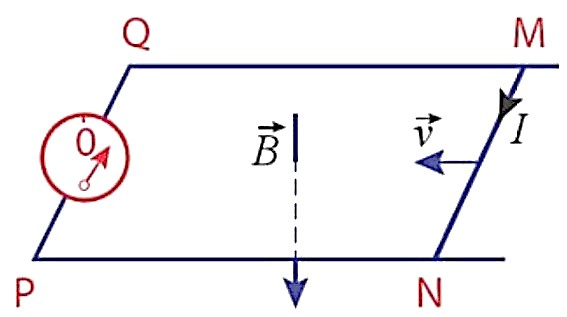
\includegraphics[width=0.4\linewidth]{figs/VN12-Y24-PH-SYL-022-1}
	\end{center}
	Khi đoạn dây dẫn chuyển động với tốc độ $\vec{v}$, suất điện động cảm ứng trong đoạn dây:
	\begin{equation}
		\left|e_c\right|=\left|\dfrac{\Delta \Phi}{\Delta t}\right|
	\end{equation}
	\begin{itemize}
		\item Khi $\vec{v}$ và $\vec{B}$ cùng vuông góc với đoạn dây chuyển động, đồng thời $\vec{v}$ vuông góc với $\vec{B}$ thì
		$$\Delta \Phi=B\Delta S=B\ell v\Delta t$$
		Như vậy:
		\begin{equation}
			\left|e_c\right|=B\ell v
		\end{equation}
		\item Nếu $\vec{v}$ và $\vec{B}$ cùng vuông góc với đoạn dây chuyển động, nhưng $\vec{v}$ tạo với $\vec{B}$ một góc $\theta$ thì:
		\begin{equation}
			\left|e_c\right|=B\ell v\sin\theta
		\end{equation}
	\end{itemize}
	\begin{noidung}{Quy tắc bàn tay phải để xác định chiều dòng điện cảm ứng trong đoạn dây chuyển động trong từ trường đều}
		Đặt bàn tay phải hứng các đường sức từ, ngón tay cái choãi ra $\SI{90}{\degree}$ hướng theo chiều chuyển động của đoạn dây, khi đó đoạn dây dẫn đóng vai trò như một nguồn điện, chiều từ cổ tay đến các ngón tay còn lại chỉ chiều dòng điện cảm ứng trên đoạn dây.
	\end{noidung}
\end{tomtat}
\subsection{Ví dụ minh hoạ}
\begin{dang}{Xác định suất điện động cảm ứng trong một đoạn dây dẫn chuyển động}
	\end{dang}
\begin{vd}
Thanh kim loại AB dài $\SI{20}{\centi\meter}$ kéo trượt đều trên hai thanh ray kim loại nằm ngang như hình vẽ. Các dây nối nhau bằng điện trở $R=\SI{3}{\ohm}$. Vận tốc của thanh AB là $\SI{12}{\meter/\second}$. Hệ thống đặt trong từ trường đều có $B=\SI{0.4}{\tesla}$, $\vec{B}$ vuông góc với mạch điện.
\begin{center}
	\begin{tikzpicture}
		\coordinate (O) at (0,0);
		\coordinate (A) at (2,1.5);
		\coordinate (B) at (2,-1.5);
		\coordinate (C) at (-4,0);
		\draw[line width=1.5pt] (A)--++(-6,0)--++(0,-3)--(B);
		\node[draw, rectangle, line width=1.5pt, fill=white, minimum height=2cm, minimum width=0.5cm, anchor=center] at (C){};
		\draw[blue, line width=1.5pt, -stealth] (O)--+(2,0);
		\draw[line width=5pt] (O)--+(0,2)--+(0,-2);
		\node[right] at ($(C)+(0.25,0)$) {$R$};
		\node[red] at ($(O)!0.5!(C)$) {\LARGE$\otimes$};
		\node[red, below] at ($(O)!0.5!(C)-(0,0.25)$) {$\vec{B}$};
		\node[blue, above] at ($(O)+(2,0)$) {$\vec{v}$};
		\node[above right] at ($(O)+(0,1.5)$) {B};
		\node[below right] at ($(O)-(0,1.5)$) {A};
	\end{tikzpicture}
\end{center}
\begin{enumerate}[label=\alph*)]
	\item Tính độ lớn suất điện động cảm ứng xuất hiện trong khung.
	\item Xác định chiều và tính cường độ dòng điện cảm ứng chạy qua đoạn mạch.
\end{enumerate}	
\loigiai{\begin{enumerate}[label=\alph*)]
		\item Độ lớn suất điện động cảm ứng trong thanh:
		$$\left|e_c\right|=B\ell v\sin\theta=\left(\SI{0.4}{\tesla}\right)\cdot\left(\SI{0.2}{\meter}\right)\cdot\left(\SI{12}{\meter/\second}\right)\cdot\sin\SI{90}{\degree}=\SI{0.96}{\volt}.$$
		\item Cường độ dòng điện cảm ứng trong mạch:
		$$i_c=\dfrac{\left|e_c\right|}{R}=\SI{0.32}{\ampere}.$$
		Áp dụng quy tắc bàn tay phải suy ra chiều của dòng điện cảm ứng đi qua thanh AB có chiều từ A đến B.
\end{enumerate}}
\end{vd}
% =========================================
\begin{vd}
	Cho mạch điện có sơ đồ như hình vẽ, nguồn điện có suất điện động $\calE=\SI{1.5}{\volt}$, điện trở trong $r=\SI{0.1}{\ohm}$, thanh MN có chiều dài $\SI{1}{\meter}$ và có điện trở $R=\SI{2.9}{\ohm}$. Từ trường $\vec{B}$ có phương vuông góc với mặt phẳng khung và hướng vào trong khung như hình vẽ, có độ lớn $B=\SI{0.1}{\tesla}$. Thanh MN có điện trở không đáng kể.
	\begin{center}
		\begin{tikzpicture}
			\coordinate (O) at (0,0);
			\coordinate (A) at (2,1.5);
			\coordinate (B) at (2,-1.5);
			\coordinate (C) at (-2,1.5);
			\coordinate (D) at (-4,0);
			\draw[line width=1.5pt] (A)--++(-6,0)--++(0,-3)--(B);
			\node[draw,line width=1.5pt, shape=circle, radius=2.5cm, fill=orange!15!white, anchor=center] at (C){\color{red}A};
			\node[draw,line width=1.5pt,white, rectangle,fill=white,minimum height=0.2cm,minimum width=1.5cm, anchor=center] at (D){};
			\draw[line width=1.5pt] ($(D)+(0,0.1)$)--+(0.5,0)--+(-0.5,0);
			\draw[line width=2.5pt] ($(D)-(0,0.1)$)--+(0.25,0)--+(-0.25,0);
			\draw[blue, line width=1.5pt, -stealth] (O)--+(2,0);
			\draw[line width=5pt] (O)--+(0,2)--+(0,-2);
			\node[red] at ($(C)-(0,1.5)$) {\LARGE$\otimes$};
			\node[red, below] at ($(C)-(0,1.65)$) {$\vec{B}$};
			\node[blue, above] at ($(O)+(2,0)$) {$\vec{v}$};
			\node[above right] at ($(O)+(0,1.5)$) {N};
			\node[below right] at ($(O)-(0,1.5)$) {M};
			\node[left] at ($(D)-(0.5,0)$) {$\calE, r$};
		\end{tikzpicture}
	\end{center}
	\begin{enumerate}[label=\alph*)]
		\item Ampere kế chỉ bao nhiêu khi MN đứng yên? Tính độ lớn lực từ tác dụng lên thanh MN khi đó.
		\item Ampere kế chỉ bao nhiêu khi MN di chuyển về phía phải với tốc độ $v=\SI{3}{\meter/\second}$ sao cho hai đầu MN luôn tiếp xúc với hai thanh đỡ bằng kim loại? Tính độ lớn lực từ tác dụng lên thanh MN khi đó.
		\item Muốn ampere kế chỉ số $0$ phải để thanh MN di chuyển về phía nào, với vận tốc là bao nhiêu?
	\end{enumerate}
	\loigiai{\begin{enumerate}[label=\alph*)]
			\item Khi thanh MN đứng yên thì trong mạch không có dòng điện cảm ứng nên số chỉ ampere kế là
			$$I=\dfrac{\calE}{R+r}=\dfrac{\SI{1.5}{\volt}}{\SI{3}{\ohm}}=\SI{0.5}{\ampere}.$$
			Độ lớn lực từ tác dụng lên thanh MN:
			$$F=I\ell B=\left(\SI{0.5}{\ampere}\right)\cdot\left(\SI{1}{\meter}\right)\cdot\left(\SI{0.1}{\tesla}\right)=\SI{0.05}{\newton}.$$
			\item Khi thanh MN chuyển động về phía phải thì trong mạch xuất hiện dòng điện cảm ứng có chiều từ M đến N và có độ lớn:
			$$i_c=\dfrac{e_c}{R+r}=\dfrac{B\ell v}{R+r}=\dfrac{\left(\SI{0.1}{\tesla}\right)\cdot\left(\SI{1}{\meter}\right)\cdot\left(\SI{3}{\meter/\second}\right)}{\SI{3}{\ohm}}=\SI{0.1}{\ampere}.$$
			Do $i_c$ ngược chiều với dòng điện do nguồn tạo ra nên cường độ dòng điện qua ampere kế:
			$$I_A=I-i_c=\SI{0.4}{\ampere}.$$
			Lực từ tác dụng lên thanh MN:
			$$F=I_A\ell B=\SI{0.04}{\newton}.$$
			\item Muốn ampere kế chỉ số 0 thì $i_c$ phải có độ lớn bằng $I=\SI{0.5}{\ampere}$ và ngược chiều với $I$. Như vậy, thanh MN phải di chuyển từ trái sang phải.\\
			Tốc độ chuyển động của thanh MN lúc này:
			$$i_c=\dfrac{B\ell v'}{R+r}\Rightarrow v'=\dfrac{i_c\left(R+r\right)}{B\ell}=\SI{15}{\meter/\second}.$$
	\end{enumerate}	}
\end{vd}

\begin{dang}{Chuyển động của đoạn dây dẫn mang dòng điện trong từ trường đều}
	\end{dang}
\begin{vd}
	Hai thanh kim loại song song, thẳng đứng có điện trở không đáng kể, một đầu nối vào điện trở $R=\SI{0.5}{\ohm}$. Một đoạn dây dẫn AB, độ dài $\ell=\SI{14}{\centi\meter}$, khối lượng $m=\SI{2}{\gram}$, điện trở $r=\SI{0.5}{\ohm}$ tì vào hai thanh kim loại. Ban đầu người ta giữ cố định dây AB rồi thả cho nó tự do trượt không ma sát xuống dưới và luôn vuông góc với hai thanh kim loại. Toàn bộ hệ thống đặt trong từ trường đều có hướng vuông góc với mặt phẳng hai thanh kim loại có cảm ứng từ $B=\SI{0.2}{\tesla}$. Lấy $g=\SI{9.8}{\meter/\second^2}$.
	\begin{center}
		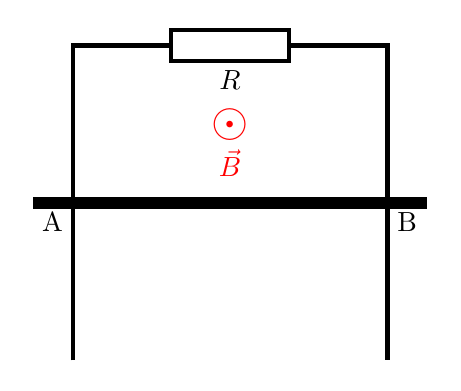
\begin{tikzpicture}
			\coordinate (A) at (0,0);
			\coordinate (B) at (4,0);
			\draw[line width=1.5pt] (0,-2)--++(0,4)--++(4,0)--++(0,-4);
			\node[draw, rectangle,fill=white, line width=1.5pt, minimum height=0.4cm, minimum width=1.5cm] at (2,2) {};
			% Thanh AB
			\draw[line width=4pt] (-0.5,0)--(4.5,0);
			
			\node[below] at(2,1.8) {$R$};
			\node[below left] at(A) {A};
			\node[below right] at(B) {B};
			\node[red] at (2,1) {\LARGE$\odot$};
			\node[red,below] at (2,0.8) {$\vec{B}$};
		\end{tikzpicture}
	\end{center}
	\begin{enumerate}[label=\alph*)]
		\item Xác định chiều dòng điện qua điện trở $R$.
		\item Chứng minh rằng lúc đầu thanh AB chuyển động nhanh dần, sau một thời gian chuyển động thì thanh AB chuyển động thẳng đều. Tính tốc độ chuyển động thẳng đều ấy và tính hiệu điện thế giữa hai đầu A, B.
		\item Bây giờ đặt hai thanh kim loại nghiêng với mặt phẳng nằm ngang một góc $\alpha=\SI{60}{\degree}$. Độ lớn và chiều của $\vec{B}$ vẫn như cũ. Tính tốc độ $v$ của chuyển động đều của thanh AB và $U_\text{AB}$.
	\end{enumerate}
	\loigiai{
	\begin{enumerate}[label=\alph*)]
		\item Do thanh đi xuống nên từ thông qua mạch tăng. Áp dụng định luật Lenz, dòng điện cảm ứng sinh ra $\vec{B}_c$ ngược chiều $\vec{B}$.\\
		Áp dụng quy tắc nắm bàn tay phải, $i_c$ có chiều từ B đến A.
		\begin{center}
			\begin{tikzpicture}
				\coordinate (A) at (0,0);
				\coordinate (B) at (4,0);
				\draw[line width=1.5pt, decoration={markings, mark=at position 0.4 with {\arrow{stealth}}},
				postaction={decorate}] (0,-2)--++(0,4)--++(4,0)--++(0,-4);
				\node[draw, rectangle,fill=white, line width=1.5pt, minimum height=0.4cm, minimum width=1.5cm] at (2,2) {};
				% Thanh AB
				\draw[line width=4pt
				] (4.5,0)--(-0.5,0);
				
				\node[below] at(2,1.8) {$R$};
				\node[below left] at(A) {A};
				\node[below right] at(B) {B};
				\node[red] at (3,1) {\LARGE$\odot$};
				\node[red,below] at (3,0.8) {$\vec{B}$};
				\node[blue] at (1,1) {\LARGE$\otimes$};
				\node[blue,below] at (1,0.8) {$\vec{B}_c$};
				\node[above left, blue] at(1,2) {$i_c$};
			\end{tikzpicture}
		\end{center}
		\item Ngay sau khi buông, thanh AB chỉ chịu tác dụng của trọng lực $\vec{P}=m\vec{g}$ nên thanh chuyển động nhanh dần $\rightarrow v$ tăng dần.\\
		Đồng thời, trong mạch xuất hiện dòng điện cảm ứng $i_c$ nên thanh AB chịu thêm tác dụng của lực từ $F=i_c\ell B$ có hướng đi lên.\\
		Mặt khác, suất điện động cảm ứng xuất hiện bên rong AB là $e_c=B\ell v$ nên
		$$i_c=\dfrac{e_c}{R+r}=\dfrac{B\ell v}{R+r}\Rightarrow F=\dfrac{B^2\ell^2v}{R+r}.$$
		Cho nên khi $v$ tăng dần thì $F$ tăng dần $\rightarrow$ tồn tại thời điểm mà $F=P$. Khi đó, thanh chuyển động thẳng đều.\\
		Khi thanh chuyển động đều thì:
		$$F=mg\Rightarrow \dfrac{B^2\ell^2v}{R+r}=mg\Rightarrow v=\dfrac{\left(R+r\right)mg}{B^2\ell^2}=\SI{25}{\meter/\second}.$$
		Hiệu điện thế giữa hai đầu thanh AB khi đó:
		$$U_\text{AB}=i_cR=\dfrac{B\ell v}{R+r}\cdot R=\SI{0.35}{\volt}.$$
		\item Khi để nghiêng hai thanh kim loại, ta có:
		\begin{center}
			\begin{tikzpicture}
				\coordinate (O) at (0,0);
				\coordinate (A) at ($(O)+(60:2.5)+(150:0.2)$);
				\coordinate (B) at ($(O)+(60:4)$);
				\coordinate (C) at ($(O)+(0:4)$);
				\coordinate (D) at (4,1.5);
				\draw[line width=1.5pt] (O)--(B);
				\draw[line width=1.5pt] (O)--(C);
				\tkzMarkAngle[size=0.75cm,color=blue, line width=1.5pt](C,O,B);
				\tkzLabelAngle[color=blue,pos=1.0](C,O,B){$\alpha$}
				
				\draw[line width=1.5pt, purple, dashed] ($(D)+(-120:1)$)--($(D)+(-2,0)$);
				\draw[line width=1.5pt, purple, dashed] ($(D)+(150:1.732)$)--($(D)+(-2,0)$);
				\draw[line width=1.5pt, purple, -stealth] (D)--+(-2,0);
				\draw[line width=1.5pt, purple, -stealth] (D)--+(150:1.732);
				\draw[line width=1.5pt, purple, -stealth] (D)--+(-120:1);
				\node[left, purple] at ($(D)+(-2,0)$)  {$\vec{B}$};
				\node[right, purple] at ($(D)+(-120:1)$)  {$\vec{B}_2$};
				\node[above, purple] at ($(D)+(150:1.732)$)  {$\vec{B}_1$};
				% Lực
				\draw[line width=2pt, red, -stealth] (A)--+(0,-2);
				\draw[line width=2pt, green!75!black, -stealth] (A)--+(60:1.5);
				\draw[line width=2pt, black, -stealth] (A)--+(150:1.5);
				\node[black, circle, fill=white, inner sep=0pt, minimum size=0pt] at (A) {\LARGE$\otimes$};
				\node[right,red] at ($(A)+(0,-2)$) {$\vec{P}$};
				\node[above,green!75!black] at ($(A)+(60:1.5)$) {$\vec{F}$};
				\node[above,black] at ($(A)+(150:1.5)$) {$\vec{N}$};
			\end{tikzpicture}
		\end{center}
		Thanh chuyển động đều khi:
		$$F=mg\sin\alpha\Rightarrow \dfrac{\left(B\sin\alpha\right)^2\ell^2v}{R+r}=mg\sin\alpha $$
		$$\Rightarrow v=\dfrac{\left(R+r\right)mg\sin\alpha}{\left(B\sin\alpha\right)^2\ell^2}=\dfrac{\left(\SI{0.5}{\ohm}+\SI{0.5}{\ohm}\right)\cdot\left(\SI{2E-3}{\kilogram}\right)\cdot\left(\SI{9.8}{\meter/\second^2}\right)\cdot\sin\SI{60}{\degree}}{\left[\left(\SI{0.2}{\tesla}\right)\sin\SI{60}{\degree}\right]^2\cdot\left(\SI{0.14}{\meter}\right)^2}=\SI{28.87}{\meter/\second}.$$
	\end{enumerate}	
	Hiệu điện thế giữa hai đầu thanh khi đó là
	$$U_\text{AB}=IR=\dfrac{B\ell v\sin\alpha}{R+r}\cdot R=\dfrac{\left(\SI{0.2}{\tesla}\right)\cdot\left(\SI{0.14}{\meter}\right)\cdot\left(\SI{28.87}{\meter/\second}\right)\sin\SI{60}{\degree}}{\SI{0.5}{\ohm}+\SI{0.5}{\ohm}}\cdot\left(\SI{0.5}{\ohm}\right)=\SI{0.35}{\volt}.$$
	}
\end{vd}
\subsubsection{Trắc nghiệm nhiều phương án lựa chọn}
\setcounter{ex}{0}
\Opensolutionfile{ans}[ans/VN12-Y24-PH-SYL-021P-TN]
% ===================================================================
\begin{ex}
	Chọn phương án đúng về chiều dòng điện cảm ứng trong thanh MN.
	\begin{center}
		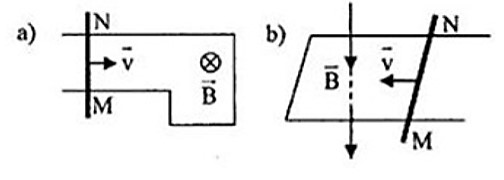
\includegraphics[width=0.4\linewidth]{figs/VN12-Y24-PH-SYL-022P-1}
	\end{center}
	\choice
	{Hình a - dòng điện cảm ứng có chiều từ N đến M, hình b - dòng điện cảm ứng có chiều từ N đến M}
	{Hình a - dòng điện cảm ứng có chiều từ M đến N, hình b - dòng điện cảm ứng có chiều từ M đến N}
	{\True Hình a - dòng điện cảm ứng có chiều từ M đến N, hình b - dòng điện cảm ứng có chiều từ N đến M}
	{Hình a - dòng điện cảm ứng có chiều từ N đến M, hình b - dòng điện cảm ứng có chiều từ M đến N}
	\loigiai{}
\end{ex}
% ===================================================================
\begin{ex}
	Đặt khung dây ABCD cạnh một dây dẫn thẳng có dòng điện trên cùng một mặt phẳng như hình
	\begin{center}
		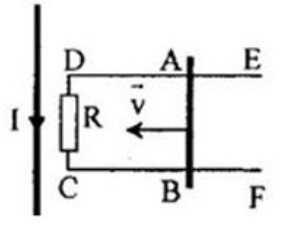
\includegraphics[width=0.25\linewidth]{figs/VN12-Y24-PH-SYL-022P-3}
	\end{center}
	Thanh AB có thể trượt trên thanh DE và CF. Điện trở $R$ không đổi và bỏ qua điện trở của các thanh. Cho AB song song với dòng điện thẳng và chuyển động thẳng đều với tốc độ không đổi. Dòng điện cảm ứng trong mạch có chiều
	\choice
	{từ  A đến B}
	{\True từ B đến A}
	{thay đổi liên tục}
	{không có dòng điện cảm ứng trong mạch}
	\loigiai{}
\end{ex}
% ===================================================================
\begin{ex}
	Đặt khung dây dẫn ABCD trong từ trường đều có chiều như hình vẽ
	\begin{center}
		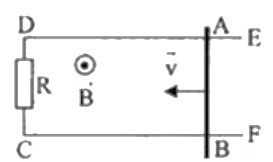
\includegraphics[width=0.25\linewidth]{figs/VN12-Y24-PH-SYL-022P-4}
	\end{center}
	Thanh AB có thể trượt. Điện trở $R$ không đổi và bỏ qua điện trở các thanh. Cường độ dòng điện cảm ứng trong mạch có biểu thức
	\choice
	{$i=\dfrac{B\ell}{vR}$}
	{$i=B\ell v$}
	{$i=\dfrac{Bv}{\ell R}$}
	{\True $i=\dfrac{B\ell v}{R}$}
	\loigiai{}
\end{ex}


% ===================================================================
\begin{ex}
	Một thanh dẫn điện dài $\SI{80}{\centi\meter}$, chuyển động trong từ trường đều với vận tốc $\SI{2}{\meter/\second}$ và vuông góc với $\vec{B}$. Biết độ lớn cảm ứng từ $B=\SI{0.4}{\tesla}$. Suất điện động cảm ứng trong thanh có độ lớn là	
	\choice
	{\True $\SI{0.64}{\volt}$}
	{$\SI{64}{\volt}$}
	{$\SI{32}{\volt}$}
	{$\SI{0.32}{\volt}$}
	\loigiai{
		Độ lớn suất điện động cảm ứng trong thanh:
		$$\left|e_c\right|=B\ell v\sin\theta=\left(\SI{0.4}{\tesla}\right)\cdot\left(\SI{0.8}{\meter}\right)\cdot\left(\SI{2}{\meter/\second}\right)\cdot\SI{90}{\degree}=\SI{0.64}{\volt}.$$	
	}
\end{ex}

% ===================================================================
\begin{ex}
	Một máy bay có chiều dài cánh $\ell=\SI{68}{\meter}$ bay theo phương ngang với vận tốc $v=\SI{720}{\kilo\meter/\hour}$. Biết thành phần thẳng đứng của cảm ứng từ Trái Đất $B=\SI{5E-5}{\tesla}$. Hiệu điện thế xuất hiện ở hai đầu cánh là
	\begin{center}
		
\includegraphics[width=0.3\linewidth]{figs/VN12-Y24-PH-SYL-022P-2}
	\end{center}
	\choice
	{$\SI{2.448}{\volt}$}
	{\True $\SI{0.68}{\volt}$}
	{$\SI{1.224}{\volt}$}
	{$\SI{1.36}{\volt}$}
	\loigiai{
		Hiệu điện thế xuất hiện ở hai cánh máy bay:
		$$U=B\ell v\sin\SI{90}{\degree}=\SI{0.68}{\volt}.$$	
	}
\end{ex}


% ===================================================================
\begin{ex}
	Một thanh dẫn điện dài $\SI{1}{\meter}$, chuyển động trong từ trường đều có cảm ứng từ $B=\SI{0.4}{\tesla}$ với vận tốc $\SI{2}{\meter/\second}$ và hợp với $\vec{B}$ một góc $\SI{30}{\degree}$. Suất điện động cảm ứng trong thanh có độ lớn là
	\choice
	{$\SI{0.4}{\volt}$}
	{$\SI{0.2}{\volt}$}
	{$\SI{0.7}{\volt}$}
	{$\SI{0.8}{\volt}$}
	\loigiai{
		Suất điện động cảm ứng suất hiện trong thanh là
		$$\left|e_c\right|=B\ell v\sin\theta=\left(\SI{0.4}{\tesla}\right)\cdot\left(\SI{1}{\meter}\right)\cdot\left(\SI{2}{\meter/\second}\right)\cdot
		\sin\SI{30}{\degree}=\SI{0.4}{\volt}.$$
	}
\end{ex}
% ===================================================================
\begin{ex}
	Một thanh dẫn điện dài $\SI{1}{\meter}$, chuyển động trong từ trường đều có cảm ứng từ $B=\SI{0.4}{\tesla}$ với vận tốc $\SI{2}{\meter/\second}$ và hợp với $\vec{B}$ một góc $\SI{30}{\degree}$. Dùng dây có điện trở không đáng kể nối hai đầu thanh với một điện trở $R=\SI{2}{\ohm}$ thành một mạch kín. Cường độ dòng điện cảm ứng qua điện trở là
	\choice
	{$\xsi{0.4\sqrt{3}}{\ampere}$}
	{$\xsi{0.2\sqrt{3}}{\ampere}$}
	{$\SI{0.4}{\ampere}$}
	{\True $\SI{0.2}{\ampere}$}
	\loigiai{
		Suất điện động cảm ứng suất hiện trong thanh là
		$$\left|e_c\right|=B\ell v\sin\theta=\left(\SI{0.4}{\tesla}\right)\cdot\left(\SI{1}{\meter}\right)\cdot\left(\SI{2}{\meter/\second}\right)\cdot
		\sin\SI{30}{\degree}=\SI{0.4}{\volt}.$$
		Cường độ dòng điện qua điện trở:
		$$I=\dfrac{\left|e_c\right|}{R}=\SI{0.2}{\ampere}.$$
	}
\end{ex}
% ===================================================================
\begin{ex}
	Thanh kim loại AB dài $\SI{20}{\centi\meter}$ kéo trượt đều trên hai thanh ray kim loại nằm ngang như hình vẽ
	\begin{center}
		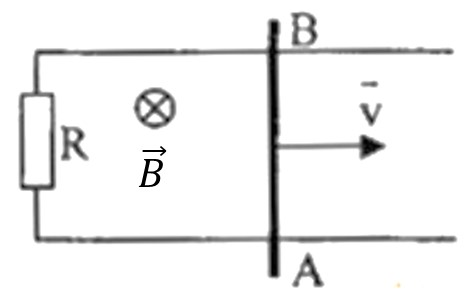
\includegraphics[width=0.25\linewidth]{figs/VN12-Y24-PH-SYL-022P-5}
	\end{center}
	Các dây nối với nhau bằng điện trở $R=\SI{3}{\ohm}$, vận tốc của thanh AB là $\SI{12}{\meter/\second}$. Hệ thống đặt trong từ trường đều có $\vec{B}$ vuông góc với mạch điện và có độ lớn cảm ứng từ $B=\SI{0.4}{\tesla}$. Chiều và độ lớn của dòng điện cảm ứng qua thanh AB là
	\choice
	{Chiều từ B đến A, $i_c=\SI{0.32}{\ampere}$}
	{\True Chiều từ A đến B, $i_c=\SI{0.32}{\ampere}$}
	{Chiều từ A đến B, $i_c=\SI{0.96}{\ampere}$}
	{Chiều từ B đến A, $i_c=\SI{0.96}{\ampere}$}
	\loigiai{
		Áp dụng định luật Lenz và quy tắc bàn tay phải ta suy ra chiều của dòng điện cảm ứng đi qua thanh AB theo chiều từ A đến B.\\
		Cường độ dòng điện cảm ứng trong thanh:
		$$i_c=\dfrac{B\ell v}{R}=\SI{0.32}{\ampere}.$$	
	}
\end{ex}
% ===================================================================
\begin{ex}
	Thanh MN chiều dài $\ell =\SI{40}{\centi\meter}$ quay đều quanh trục qua M và vuông góc với thanh trong từ trường đều $B = \SI{0.25}{\tesla}$ làm xuất hiện suất điện động cảm ứng $e_c=\SI{0.4}{\volt}$ trong thanh.
	\begin{center}
		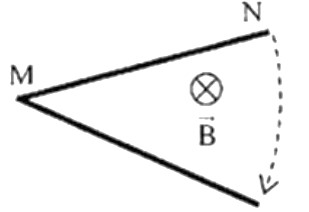
\includegraphics[width=0.25\linewidth]{figs/VN12-Y24-PH-SYL-022P-6}
	\end{center}
	Tốc độ góc của thanh là
	\choice
	{$\SI{30}{\radian/\second}$}
	{$\SI{10}{\radian/\second}$}
	{\True $\SI{20}{\radian/\second}$}
	{$\SI{40}{\radian/\second}$}
	\loigiai{
		Trong khoảng thời gian $\Delta t$ thanh quét được diện tích:
		$$\Delta S=\pi \ell^2\dfrac{\Delta \varphi}{2\pi}=\pi\ell^2\dfrac{\omega\Delta t}{2\pi}=\dfrac{\ell^2\omega}{2}\Delta t.$$
		Độ biến thiên từ thông:
		$$\Delta \Phi=B\Delta S\cos\alpha=B\Delta S$$
		Suất điện động cảm ứng:
		$$\left|e_c\right|	=\dfrac{\Delta \Phi}{\Delta t}=\dfrac{B\Delta S}{\Delta t}=\dfrac{B\dfrac{\ell^2 \omega}{2}\Delta t}{\Delta t}=\dfrac{B\ell^2\omega}{2}\rightarrow\omega=\SI{20}{\radian/\second}.$$
	}
\end{ex}
% ===================================================================
\begin{ex}
	Hai thanh kim loại song song thẳng đứng một đầu nối với tụ điện có điện dung $C=\SI{1}{\micro\farad}$. Một đoạn dây dẫn AB có độ dài $\ell=\SI{10}{\centi\meter}$, khối lượng $m=\SI{15}{\gram}$ tì vào hai thanh kim loại, tự do trượt không ma sát xuống dưới và luôn vuông góc với hai thanh kim loại trên. Hệ thống đặt trong từ trường đều vuông góc với mặt phẳng khung dây, cảm ứng từ có độ lớn $\SI{1}{\tesla}$. Bỏ qua điện trở của các đoạn dây dẫn. Lấy gia tốc trọng trường $g=\SI{10}{\meter/\second^2}$. Gia tốc của thanh AB là
	\begin{center}
		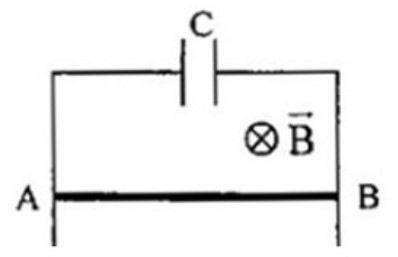
\includegraphics[width=0.3\linewidth]{figs/VN12-Y24-PH-SYL-022P-7}
	\end{center}
	\choice
	{\True $\SI{10}{\meter/\second^2}$}
	{$\SI{5}{\meter/\second^2}$}
	{$\SI{0.1}{\meter/\second^2}$}
	{$\SI{0.05}{\meter/\second^2}$}
	\loigiai{
		Thanh chịu tác dụng của trọng lực và lực từ.\\
		Ta có:
		\begin{equation}
			P-F=ma
			\label{eq: 1}
		\end{equation}
		Trong đó:
		\begin{itemize}
			\item Trọng lực $P=mg$\\
			\item Lực từ $F=I\ell B$
		\end{itemize}
		Cường độ dòng điện qua thanh:
		$$I=\dfrac{\Delta q}{\Delta t}=\dfrac{C\Delta e_c}{\Delta t}=\dfrac{CB\ell\Delta v}{\Delta t}=CB\ell a$$
		Thay vào phương trình \eqref{eq: 1} ta được:
		$$mg-CB^2\ell^2a=ma\Rightarrow a=\dfrac{mg}{CB^2\ell^2+m}=\dfrac{\left(\SI{15E-3}{\kilogram}\right)\cdot\left(\SI{10}{\meter/\second^2}\right)}{\left(\SI{e-6}{\farad}\right)\cdot\left(\SI{1}{\tesla}\right)^2\cdot\left(\SI{0.1}{\meter}\right)^2+\SI{15E-3}{\kilogram}}\approx\SI{10}{\meter/\second^2}.$$
	}
\end{ex}
% ===================================================================
\begin{ex}
	Hai thanh kim loại được đặt song song nghiêng góc $\SI{30}{\degree}$ so với phương ngang, một đầu nối với tụ điện có điện dung $C=\SI{4}{\micro\farad}$. Một đoạn dây dẫn AB có độ dài $\ell=\SI{10}{\centi\meter}$, khối lượng $m=\SI{20}{\gram}$ tì vào hai thanh kim loại, tự do trượt không ma sát. Hệ thống đặt trong từ trường đều có vector cảm ứng từ $\vec{B}$ vuông góc với mặt phẳng hai thanh ray và có độ lớn $B=\SI{1}{\tesla}$, bỏ qua điện trở của các đoạn dây.
	\begin{center}
		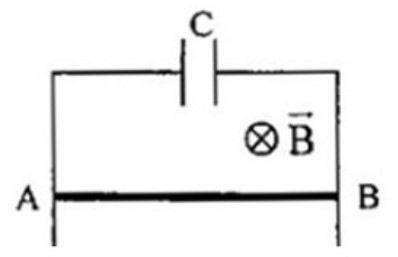
\includegraphics[width=0.3\linewidth]{figs/VN12-Y24-PH-SYL-022P-7}
	\end{center}
	Thanh AB được thả từ vị trí cách đầu dưới của hai thanh kim loại đoạn $d=\SI{5}{\centi\meter}$. Thời gian để AB bắt đầu rời khỏi thanh kim loại là
	\choice
	{$\SI{0.1}{\second}$}
	{\True $\SI{0.14}{\second}$}
	{$\SI{0.2}{\second}$}
	{$\SI{0.4}{\second}$}
	\loigiai{
		Cường độ dòng điện qua thanh 
		$$I=\dfrac{\Delta q}{\Delta t}=\dfrac{\Delta e_c}{\Delta t}=CB\ell\dfrac{\Delta v}{\Delta t}=CB\ell a.$$
		Áp dụng định luật II Newton và chiếu lên phương chuyển động của thanh AB:
		$$P\sin\alpha-F\sin\alpha=ma$$
		$$\Leftrightarrow mg\sin\alpha-CB^2\ell^2a\sin\alpha=ma$$
		$$\Rightarrow a=\dfrac{mg\sin\alpha}{m+CB^2\ell^2\sin\alpha}\approx\SI{5}{\meter/\second^2}.$$
		Thời gian thanh AB rời khỏi thanh kim loại:
		$$t=\sqrt{\dfrac{2d}{a}}\approx\SI{0.14}{\second}.$$
		
	}
\end{ex}
\Closesolutionfile{ans}
\subsubsection{Tự luận}
\setcounter{ex}{0}
\Opensolutionfile{ans}[ans/VN12-Y24-PH-SYL-021P-TL]
% ======================================================================
\begin{ex}
	Một thanh dẫn điện MN trượt trên hai thanh kim loại trong vùng từ trường đều vuông góc với hướng của cảm ứng từ như hình bên dưới. Biết $B=\SI{0.60}{\tesla}$, $\mathrm{MN}=\mathrm{PQ}=\SI{0.30}{\meter}$, toàn bộ mạch điện có điện trở $\SI{20}{\ohm}$. Thanh đang chuyển động về bên trái với tốc độ $\SI{6.0}{\meter/\second}$ và có hướng vuông góc với thanh.
	\begin{center}
		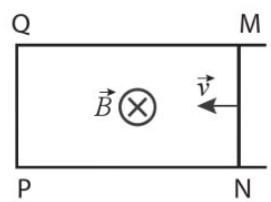
\includegraphics[width=0.25\linewidth]{figs/VN12-Y24-PH-SYL-022P-8}
	\end{center}
	Xác định:
	\begin{enumerate}[label=\alph*)]
		\item độ lớn suất điện động cảm ứng.
		\item cường độ dòng điện cảm ứng.
		\item công suất cần thiết để di chuyển thanh.
	\end{enumerate}
	\loigiai{
		\begin{enumerate}[label=\alph*)]
			\item $\left|e_c\right|=B\ell v\approx\SI{1.1}{\volt}$.
			\item $I=\dfrac{\left|e_c\right|}{R}=\SI{0.055}{\ampere}$.
			\item $\calP=\left|e_c\right|\cdot I=\SI{0.06}{\watt}$.
		\end{enumerate}	
	}
\end{ex}
% ======================================================================
\begin{ex}
	Cho mạch điện như hình vẽ: suất điện động nguồn điện $E=\SI{1.5}{\volt}$ và điện trở trong $r=\SI{0.2}{\ohm}$. Thanh MN dài $\SI{1}{\meter}$ và có điện trở $R_{\text{MN}}=\SI{2.8}{\ohm}$. Cảm ứng từ có độ lớn $B=\SI{0.1}{\tesla}$. Bỏ qua điện trở của ampe kế A.
	\begin{center}
		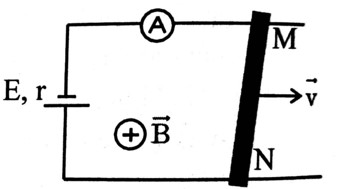
\includegraphics[width=0.25\linewidth]{figs/VN12-Y24-PH-SYL-022P-9}
	\end{center}
	\begin{enumerate}[label=\alph*)]
		\item Xác định số chỉ của ampe kế A khi:
		\begin{itemize}
			\item MN đứng yên.
			\item MN chuyển động đều về bên phải với vận tốc $v=\SI{5}{\meter/\second}$.
		\end{itemize}
		\item Muốn cho ampe kế chỉ 0 thì phải dịch chuyển MN về phía nào và với vận tốc bằng bao nhiêu?
	\end{enumerate}
	
	\loigiai{
		\begin{enumerate}[label=\alph*)]
			\item \begin{itemize}
				\item Khi MN đứng yên:
				$$I=\dfrac{E}{R_{\text{MN}}+r}=\dfrac{1,5}{2,8+0,2}=\SI{0.5}{\ampere}.$$
				\item Khi MN chuyển động, trong thanh xuất hiện suất điện động cảm ứng $e_c$:
				$$e_c=B\ell v=0,1\cdot1\cdot5=\SI{0.5}{\volt}.$$
				Cường độ dòng điện cảm ứng:
				$I_c=\dfrac{e_c}{R_{\text{MN}}+r}$.\\
				Dùng quy tắc bàn tay phải, xác định được $I_c$ cùng chiều $I$
				$$\Rightarrow I_A=I+I_c=\dfrac{E+e_c}{R_{\text{MN}}+r}=\dfrac{1,5+0,5}{2,8+0,2}=\xsi{\dfrac{2}{3}}{\ampere}.$$
			\end{itemize}
			\item Muốn $I_c$ ngược chiều thì thanh MN phải dịch chuyển về phía ngược lại (về phía trái).\\
			Để $I_A=I-I_c=0$ thì $e_c=E\Leftrightarrow Bv'\ell=1,5\Rightarrow v'=\dfrac{1,5}{B\ell}=\dfrac{1,5}{0,1\cdot1}=\SI{15}{\meter/\second}.$
		\end{enumerate}	
		
	}
\end{ex}





\Closesolutionfile{ans}